\section{Results}
\subsection{40 Minute Single Voxel Simulation}
\begin{frame}{Long Run Results}
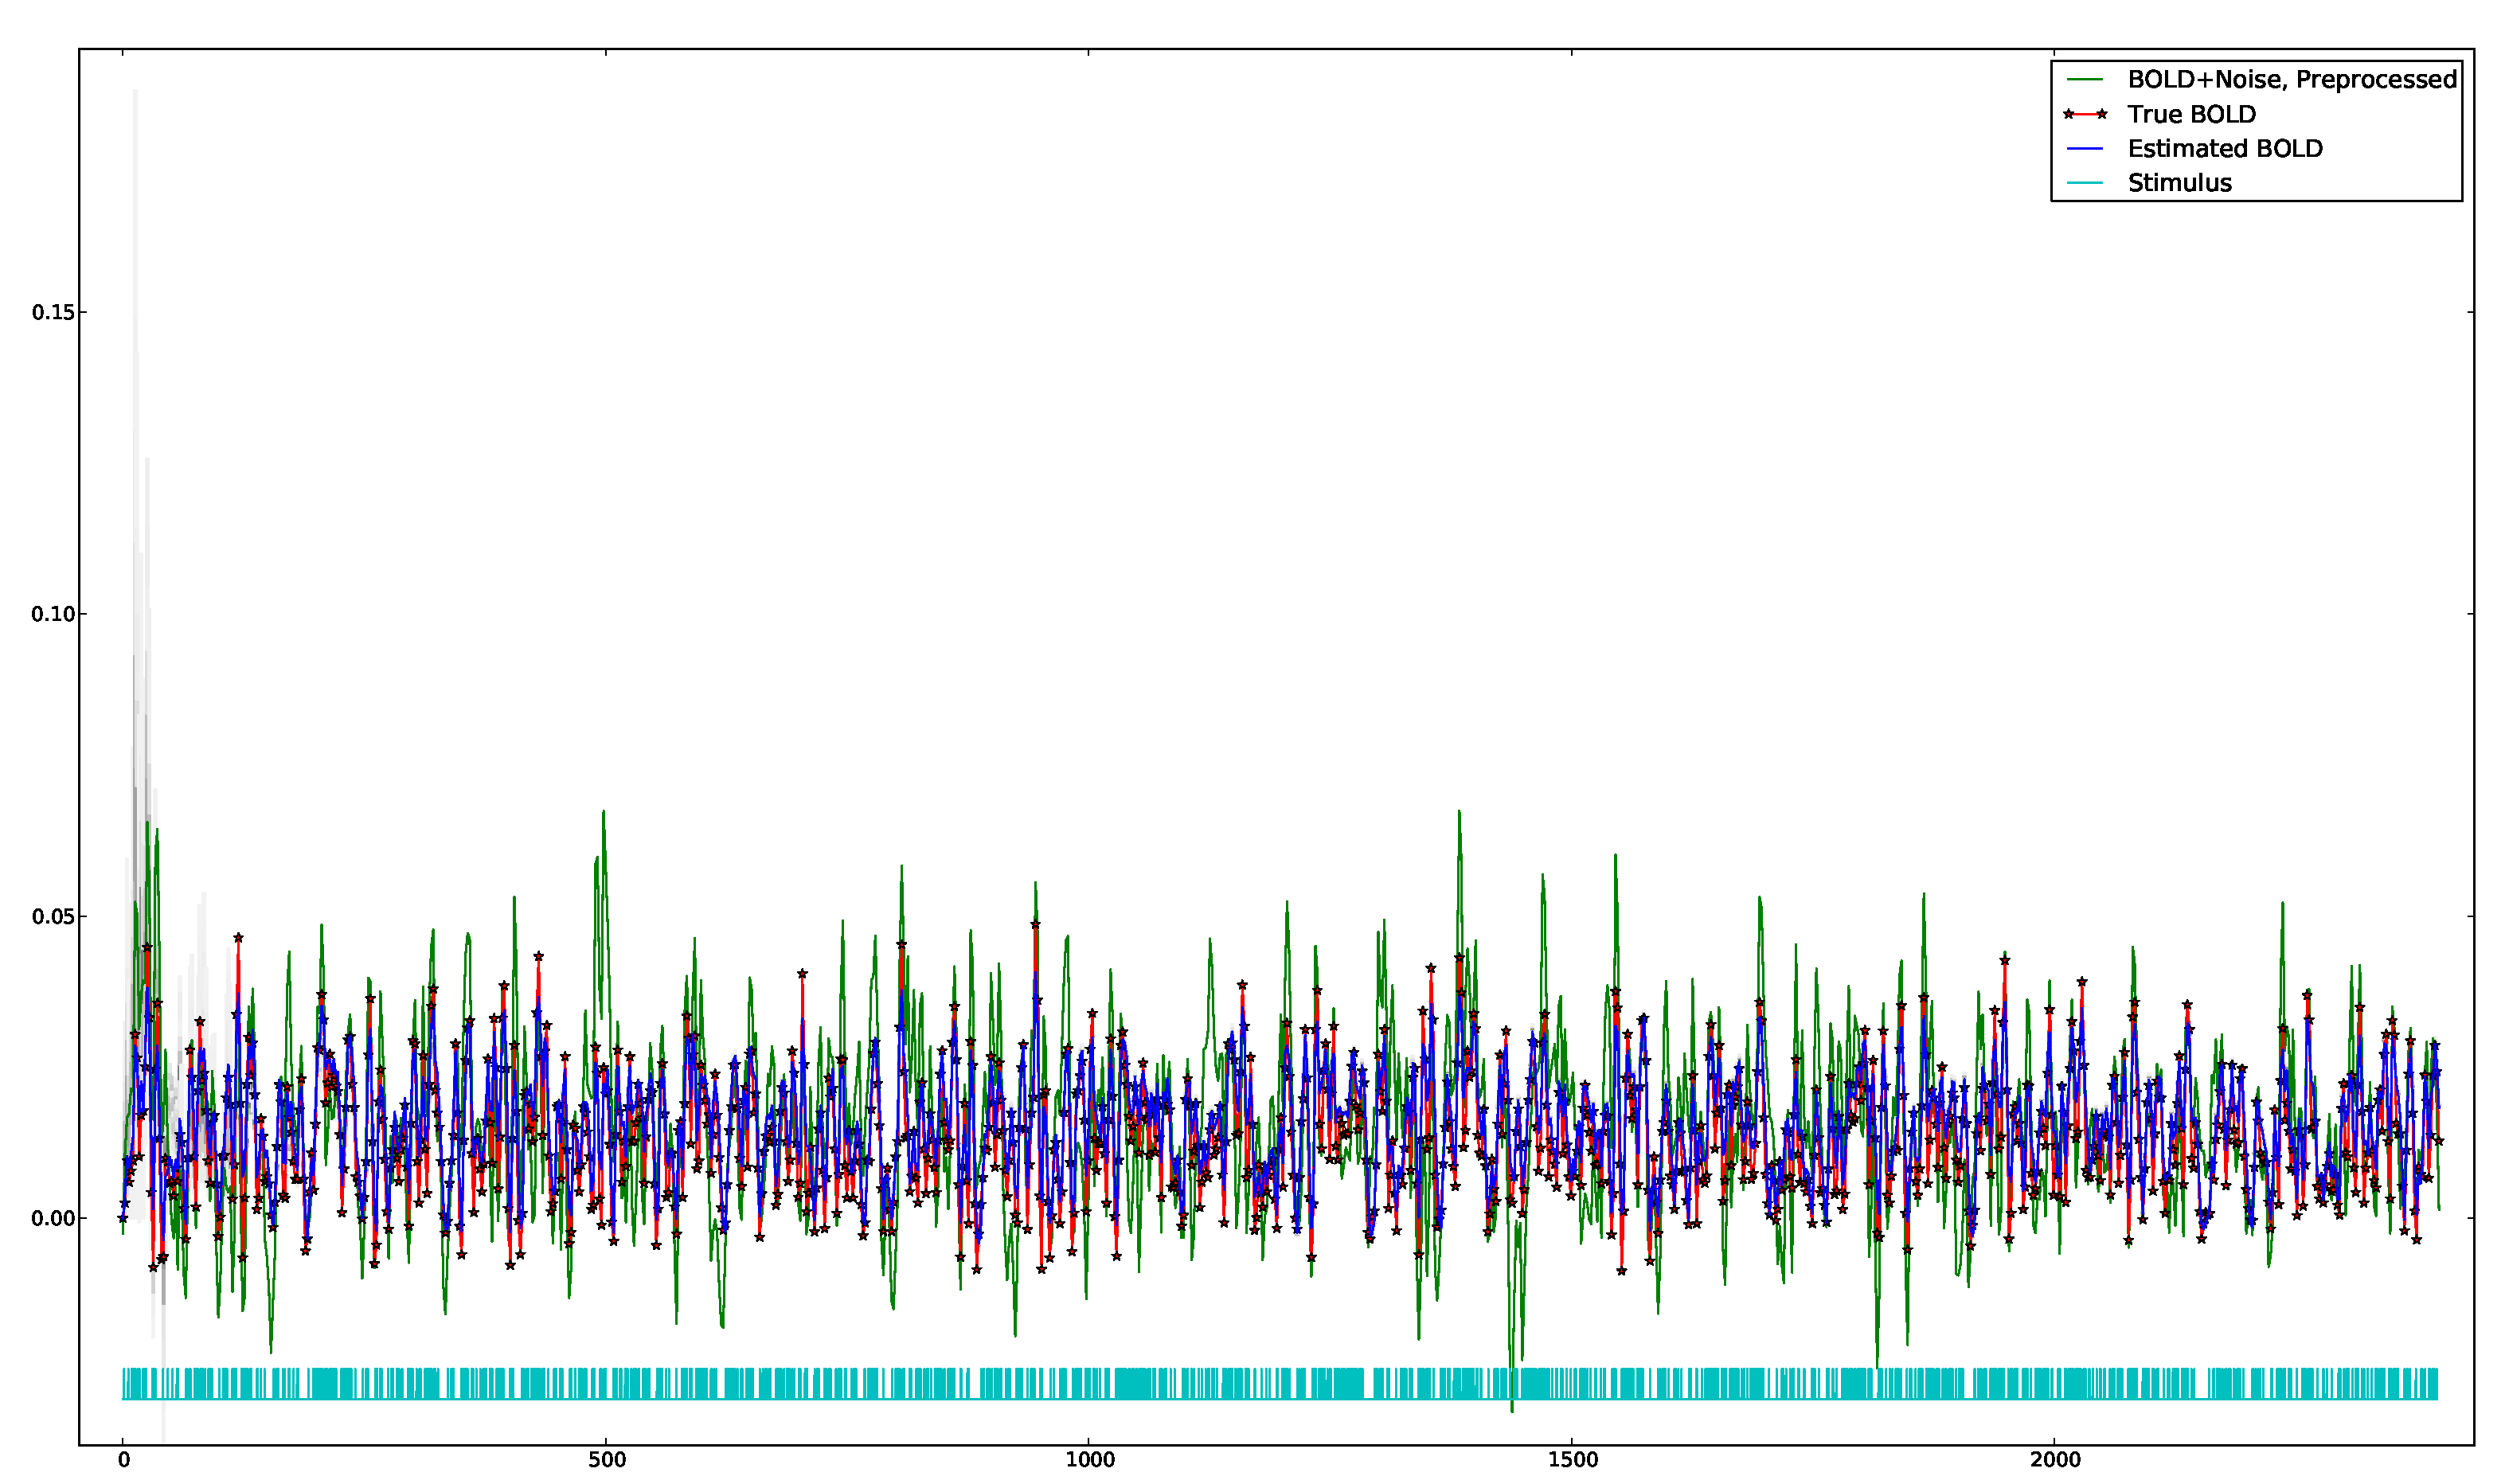
\includegraphics[width=\textwidth]{long_converge}
\note{Bars drop well before the end}
\note{Mean is good estimator}
\note{Mean comes very close to truth}
\end{frame}

\begin{frame}{Long Run Covariance and Correlation}
\centering
Estimated Parameter Covariance 

\begin{table}[t]
\tiny
\begin{tabular}{|c | c  c  c  c  c  c  c |}
\hline
  & $\tau_0$ & $\alpha$ & $E_0$    & $V_0$    & $\tau_s$ & $\tau_f$ & $\epsilon$ \\
\hline
\rowcolor[gray]{.8} $\tau_0$  & 0.0004334 & 5.2e-05 & -6.95e-05 & 3.3e-06 & 0.0001628 & -2e-07 & 0.0001798 \\
$\alpha$                      & 5.2e-05 & 7.9e-06 & -6.4e-06 & 3e-07 & 1.04e-05 & -1.92e-05 & 2.58e-05 \\
\rowcolor[gray]{.8} $E_0$     & -6.95e-05 & -6.4e-06 & 1.9e-05 & -9e-07 & -4.11e-05 & -3.24e-05 & -3.92e-05 \\
$V_0$                         & 3.3e-06 & 3e-07 & -9e-07 & 1e-07 & 1.1e-06 & 9e-07 & 1e-06 \\
\rowcolor[gray]{.8} $\tau_s$  & 0.0001628 & 1.04e-05 & -4.11e-05 & 1.1e-06 & 0.0001589 & 0.0001518 & 7.88e-05 \\
$\tau_f$                      & -2e-07 & -1.92e-05 & -3.24e-05 & 9e-07 & 0.0001518 & 0.0002966 & -2.34e-05 \\
\rowcolor[gray]{.8} $\epsilon$& 0.0001798 & 2.58e-05 & -3.92e-05 & 1e-06 & 7.88e-05 & -2.34e-05 & 0.0001966 \\
\hline
\end{tabular}
\label{tab:long_cov}
\end{table}

Estimated Parameter Correlation 

\begin{table}[t]
\tiny
\begin{tabular}{|c | c  c  c  c  c  c  |}
\hline
  & $\tau_0$ & $\alpha$ & $E_0$    & $V_0$    & $\tau_s$ & $\tau_f$  \\
\hline
\rowcolor[gray]{.8} $\tau_0$  & & & & & & \\
$\alpha$                      & 0.889884 & & & & & \\
\rowcolor[gray]{.8} $E_0$     & -0.7661395 & -0.5230723 & & & & \\
$V_0$                         & 0.6244049 & 0.4239271 & -0.7964774 & & & \\
\rowcolor[gray]{.8} $\tau_s$  & 0.6204843 & 0.295425 & -0.7481253 & 0.3440421 & & \\
$\tau_f$                      & -0.0004259 & -0.3966881 & -0.4314174 & 0.1962954 & 0.6990775 & \\
\rowcolor[gray]{.8} $\epsilon$& 0.6158116 & 0.6558179 & -0.641348 & 0.2846632 & 0.4458142 & -0.097079 \\
\hline
\end{tabular}
\note{Correlation of parameter estimates at the end of 
            \autoref{fig:long_converge}.}
\label{tab:long_corr}
\end{table}
\end{frame}

\subsection{5 Minute, Single Voxel Simulation}
\begin{frame}{Preprocessed Noisy Simulation vs. Underlying Signal}
\begin{center}
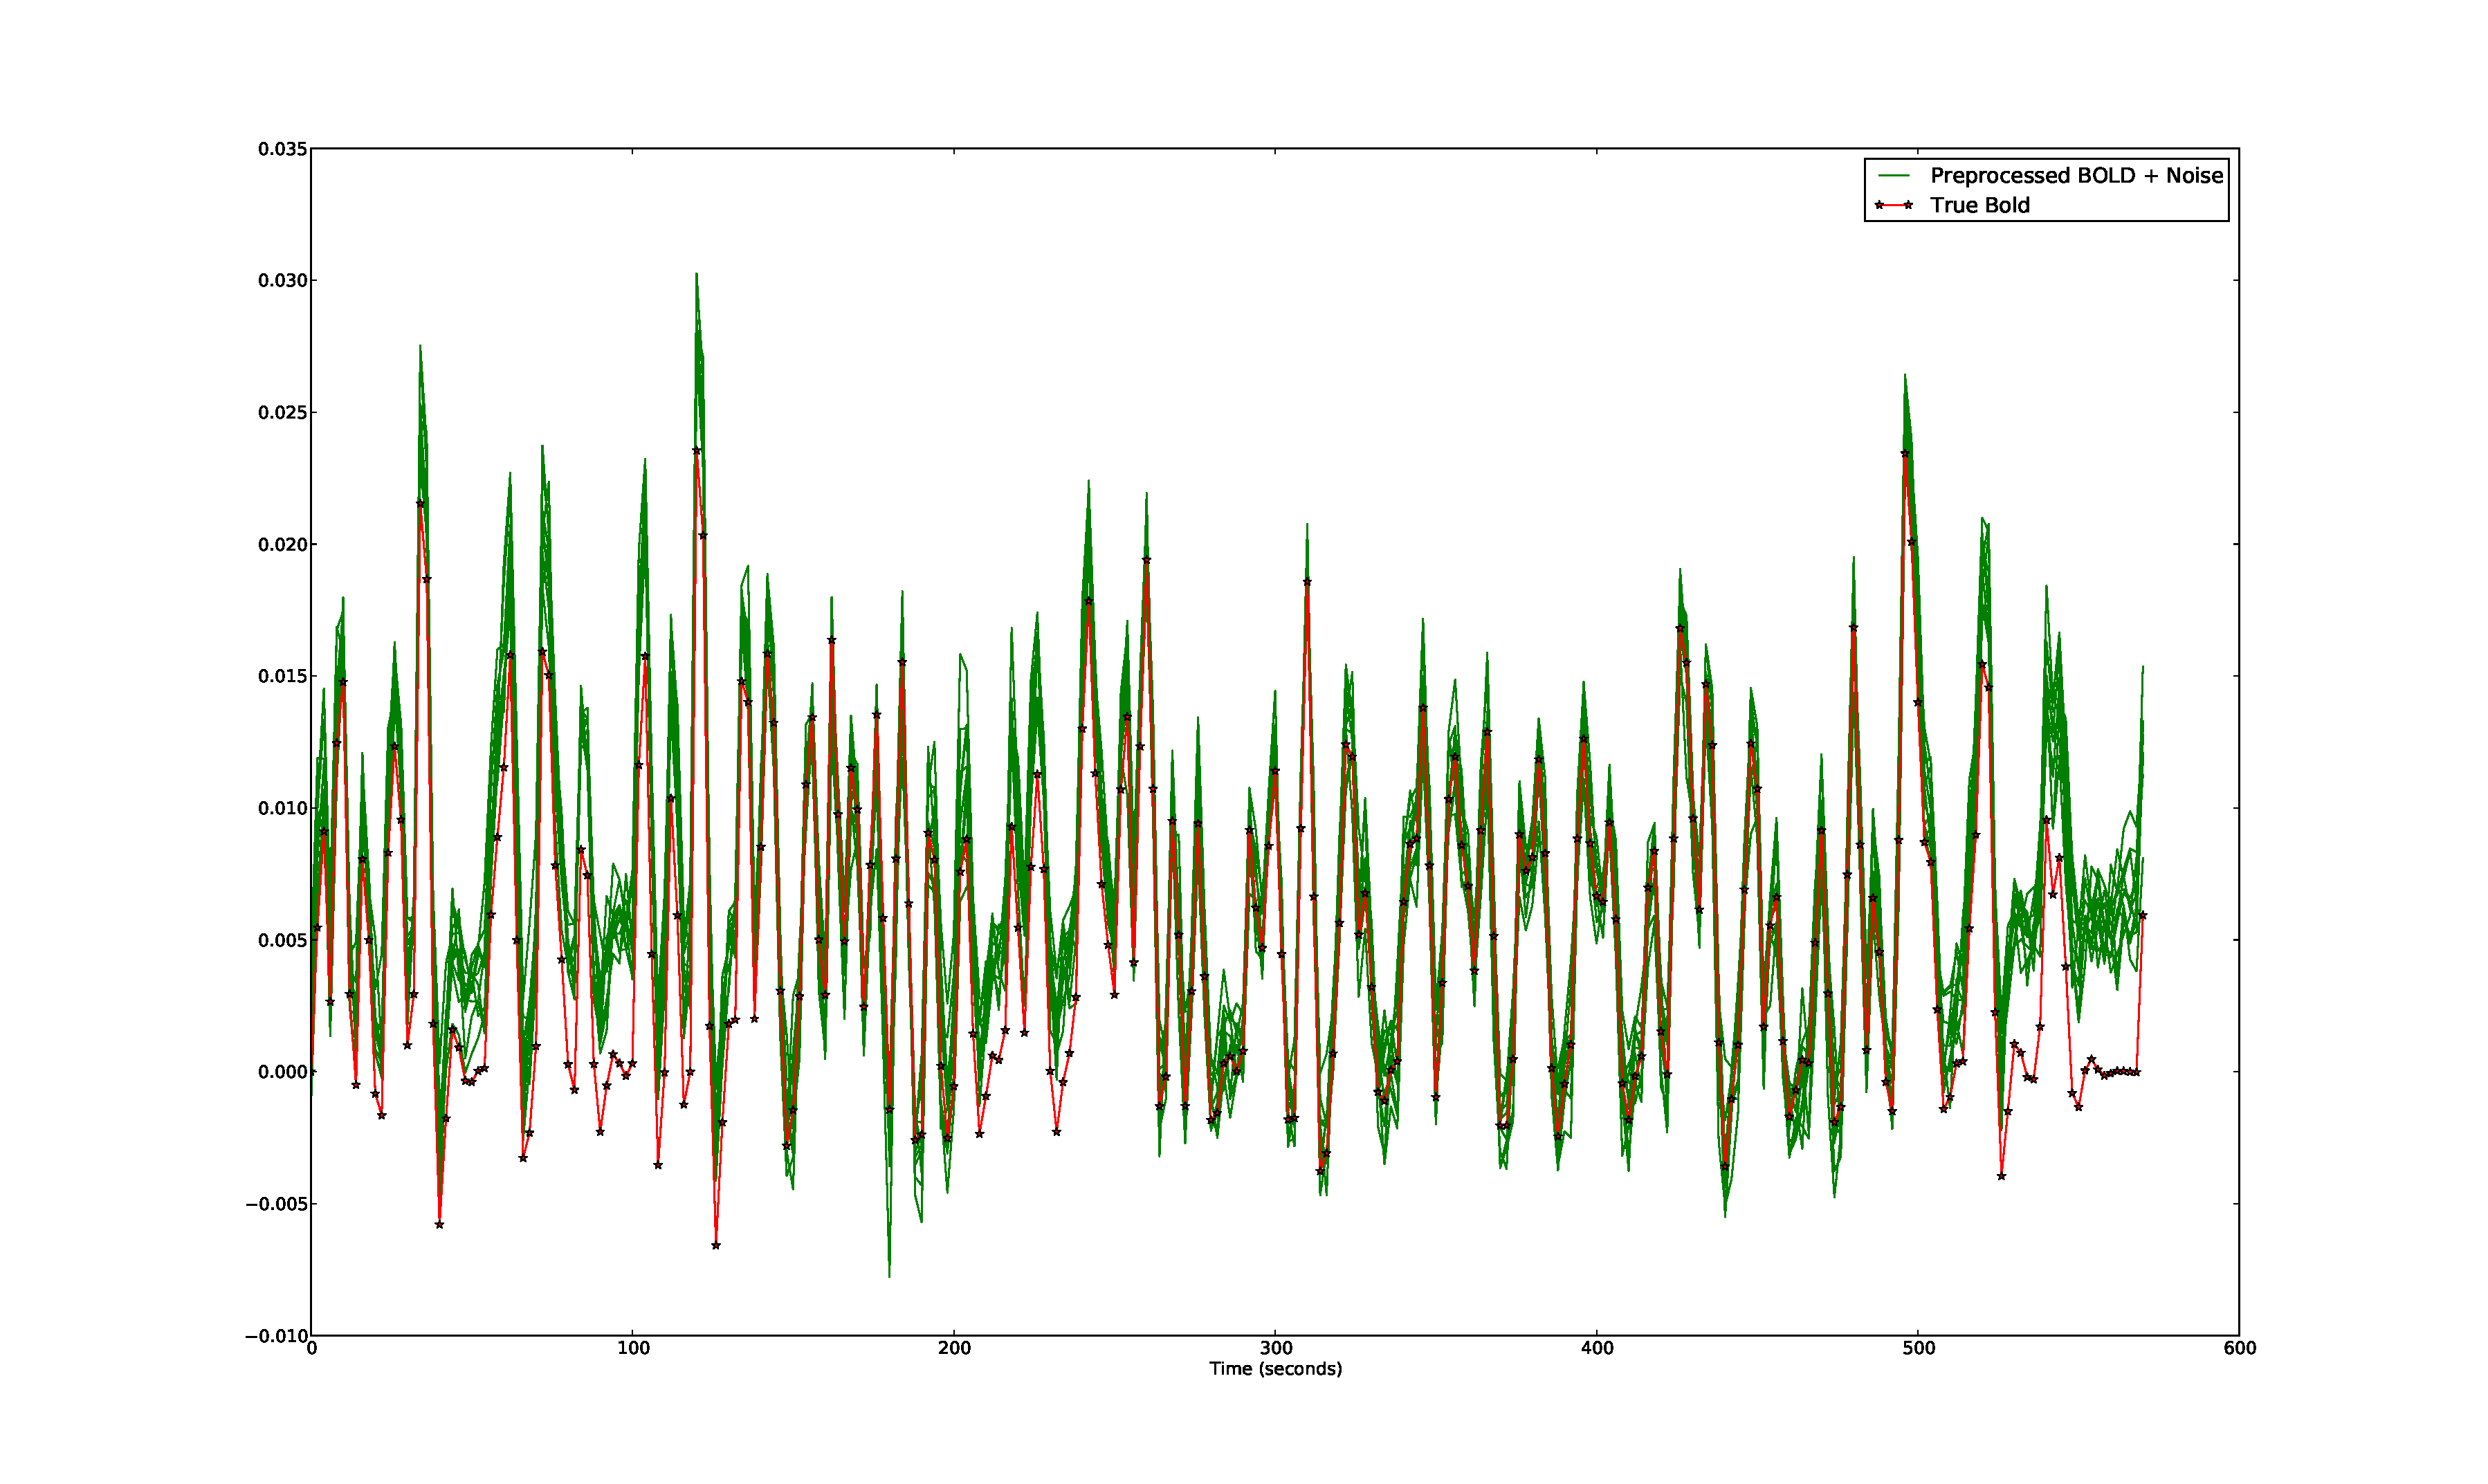
\includegraphics[clip=true,trim=6cm 2cm 5cm 3.5cm,width=.9\textwidth]
            {preprocessed_lownoise}
\end{center}
\end{frame}

\begin{frame}{Estimated vs. Underlying Signal}
\begin{center}
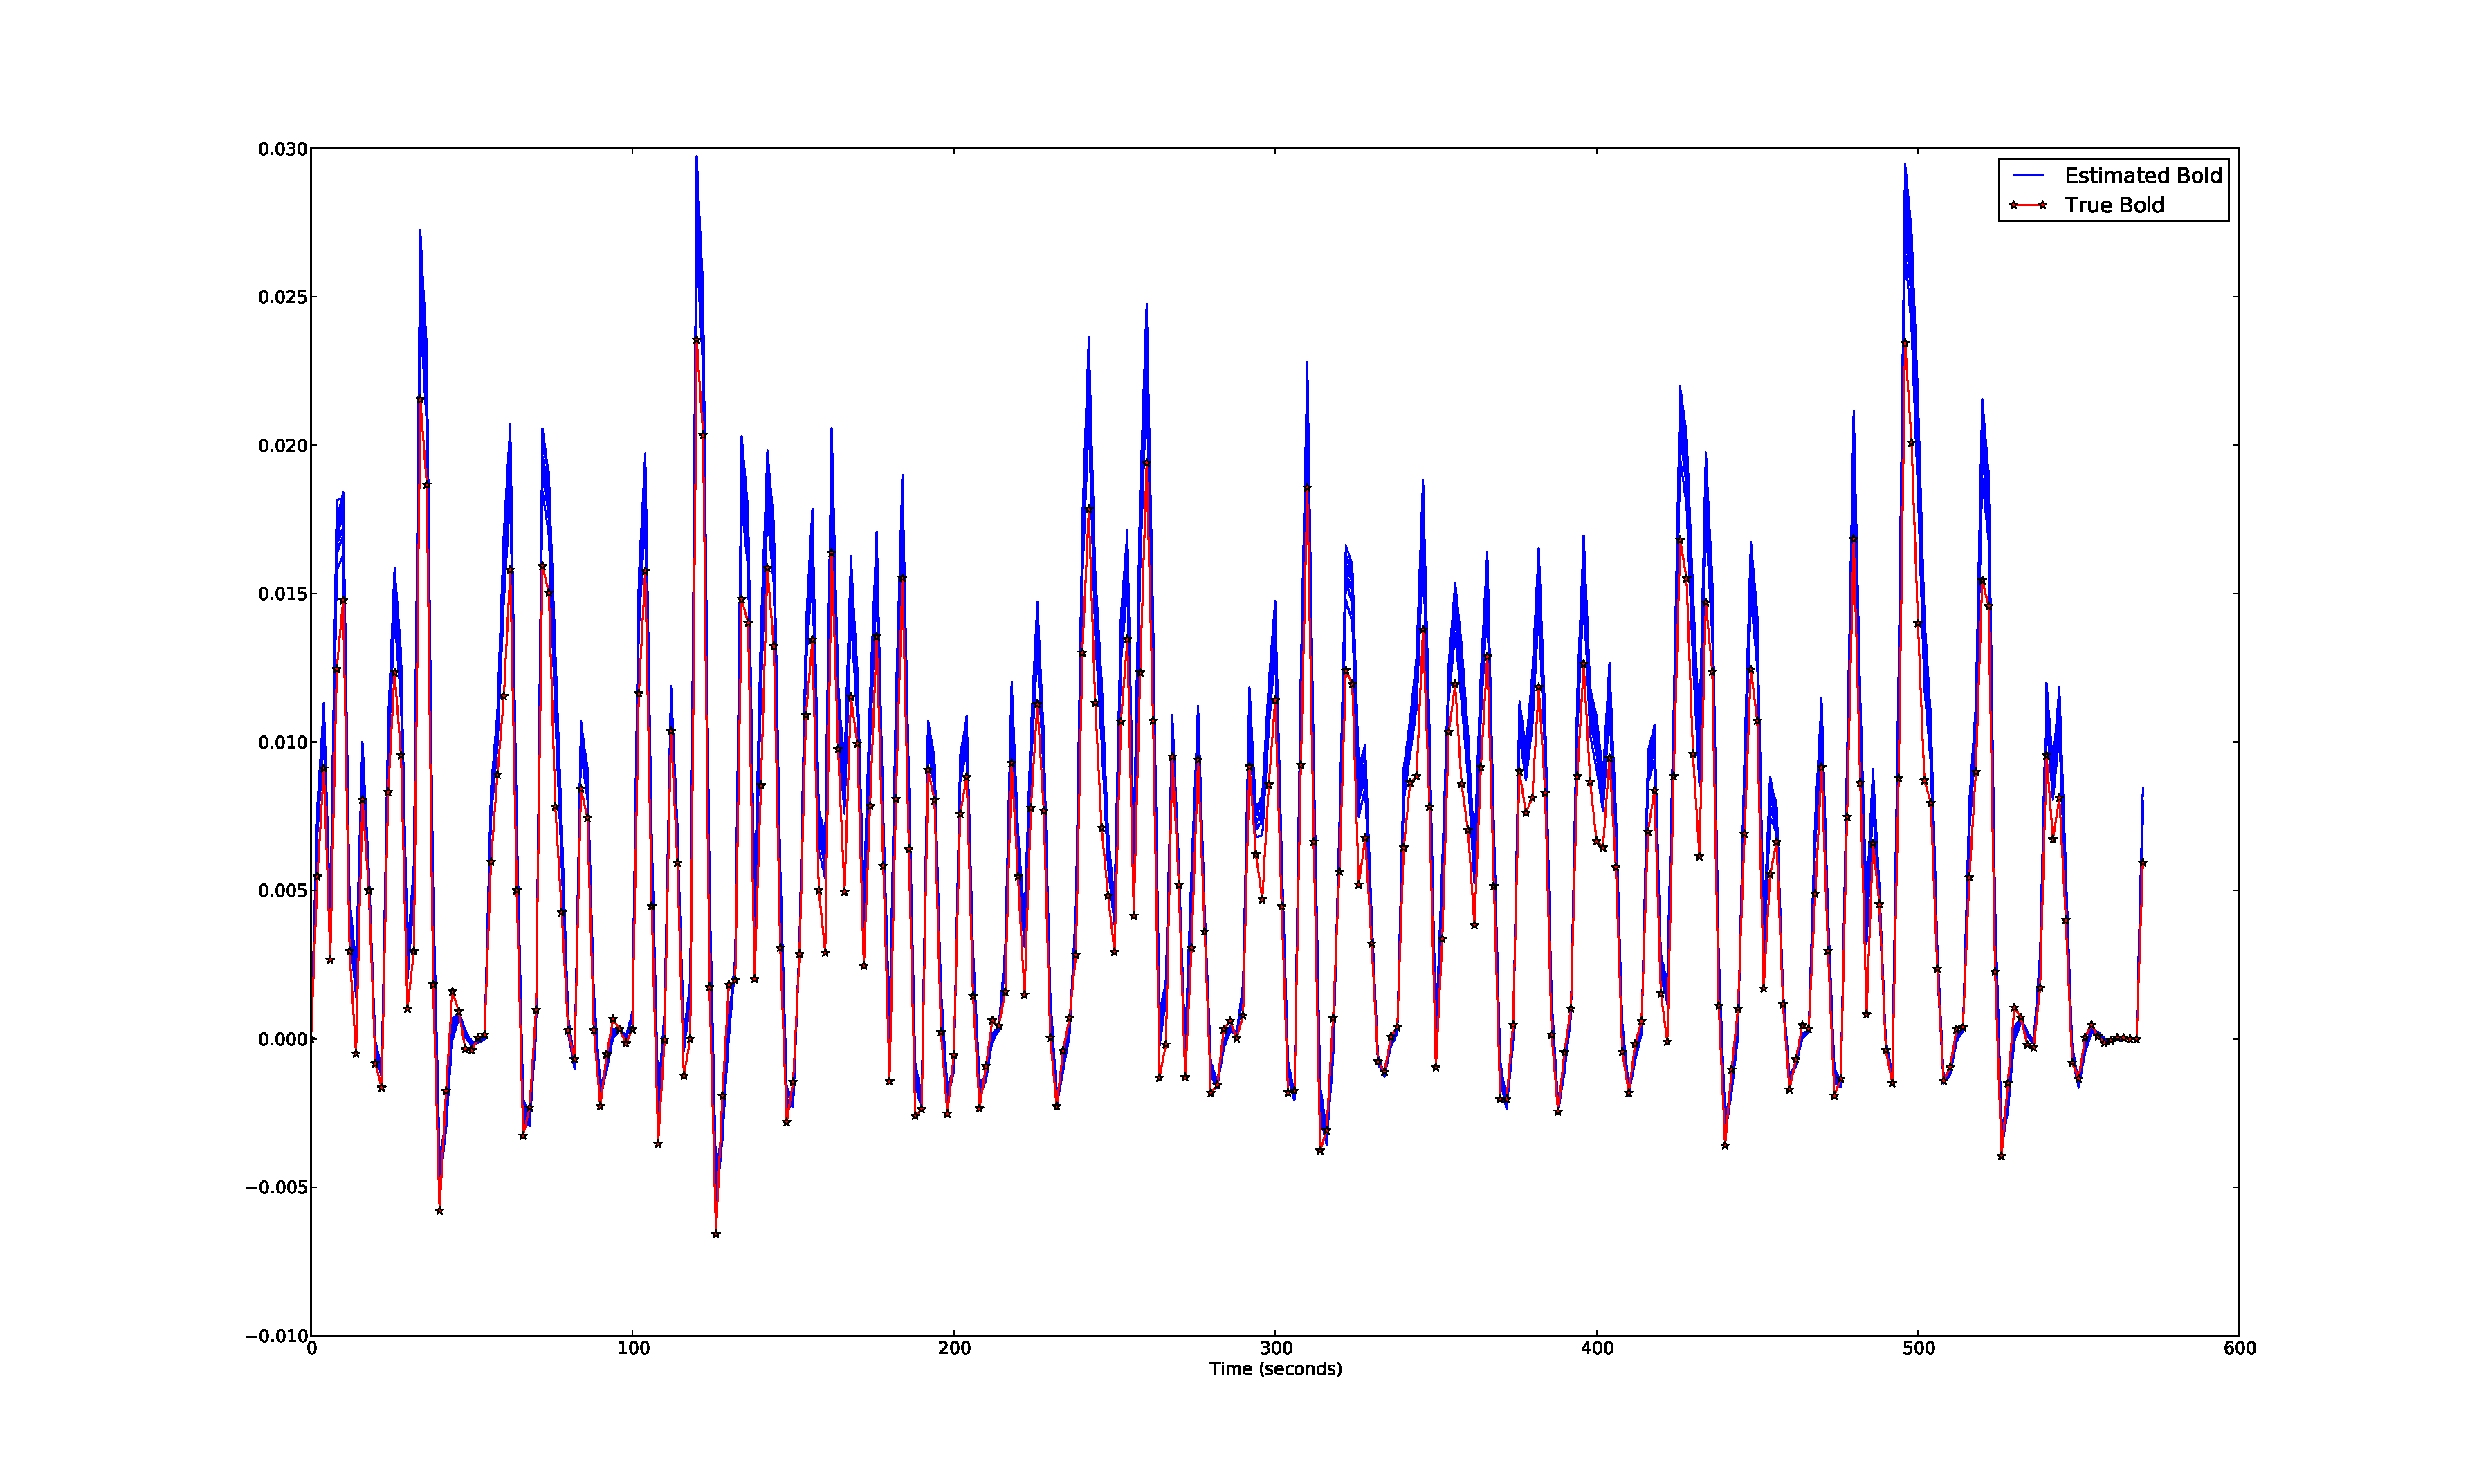
\includegraphics[clip=true,trim=6cm 2cm 5cm 3.5cm,width=.9\textwidth]
            {comparison_lownoise}
\end{center}
\end{frame}

\begin{frame}{Estimated Parameters}
\begin{table}[t]
\centering
\resizebox{\textwidth}{!}{
\begin{tabular}{|c | c | c | c | c | c | c | c | c | c |}
\hline
$\tau_0$ & $\alpha$ & $E_0$    & $V_0$    & $\tau_s$ & $\tau_f$ & $\epsilon$  & $ \sum \tau $ & Error & Residual\\
\hline
\rowcolor[gray]{.8}
1.45 & 0.3 & 0.47 & 0.044 & 1.94 & 1.99 & 1.8  & 5.38 &  & \\
\hline
\hline
1.2221 & 0.3449 & 0.3346 & 0.0714 & 1.6045 & 2.2753 & 1.5945 & 5.1019 &  0.003211  & 0.00224\\
1.3749 & 0.3318 & 0.3630 & 0.0733 & 1.6408 & 2.1030 & 1.5763 & 5.1187 &  0.003055  & 0.00223\\
1.1660 & 0.3221 & 0.3406 & 0.0822 & 1.6477 & 2.3535 & 1.2452 & 5.1672 &  0.003289  & 0.00205\\
1.2318 & 0.3271 & 0.3403 & 0.0796 & 1.6270 & 2.1852 & 1.3033 & 5.0439 &  0.002847  & 0.00147\\
1.1832 & 0.3179 & 0.3472 & 0.0821 & 1.5496 & 2.2912 & 1.2782 & 5.0240 &  0.003006  & 0.00213\\
1.1424 & 0.334  & 0.3473 & 0.0737 & 1.6221 & 2.2908 & 1.4025 & 5.0553 &  0.002833  & 0.00184\\
1.3004 & 0.3596 & 0.3564 & 0.0768 & 1.5641 & 2.1323 & 1.6034 & 4.9968 &  0.003028  & 0.00255\\
1.2401 & 0.3460 & 0.3398 & 0.0891 & 1.6499 & 2.2366 & 1.2900 & 5.1265 &  0.003044  & 0.00238\\
1.1709 & 0.3274 & 0.3464 & 0.0826 & 1.5373 & 2.2826 & 1.3783 & 4.9909 &  0.003345  & 0.0027 \\
1.1897 & 0.3434 & 0.3355 & 0.0798 & 1.5358 & 2.3075 & 1.4277 & 5.0330 &  0.003175  & 0.00244\\
1.184 &  0.3405 & 0.3502 & 0.0892 & 1.6103 & 2.2793 & 1.1645 & 5.0735 &  0.002889  & 0.00188\\
\hline                                                                               
1.2187 & 0.3359 & 0.3456 & 0.0800 & 1.599 & 2.2488 & 1.3876 & 5.0665 & 0.003066     & 0.00217\\
\hline
\end{tabular}
}
\end{table}
\end{frame}

\subsection{POSSUM Simulation}
\begin{frame}{Mutual Information Compared with SNR}
\begin{figure}
\centering
\subfigure[Regions]{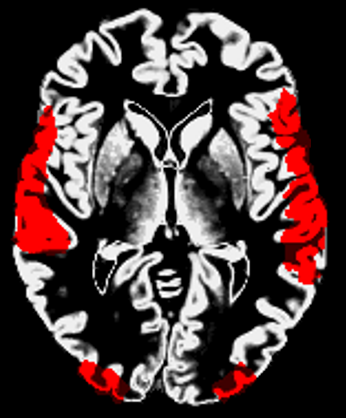
\includegraphics[height=.46\textheight]{simregions}}
\subfigure[Mutual Information]
{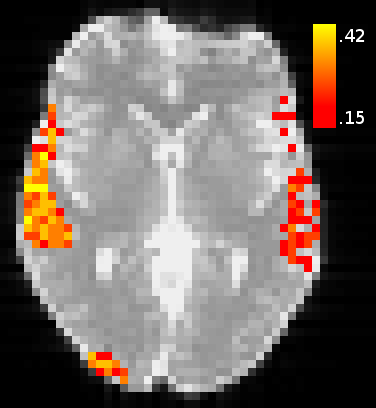
\includegraphics[height=.46\textheight]{sim_hm_15_6}}
\subfigure[SNR]{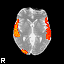
\includegraphics[height=.46\textheight]{snr_hm}}
\note{Mean SNR's Region 1: $0.8$, Region 2: $0.97$, and Region 3: $0.39$.}
\end{figure}
\end{frame}

\begin{frame}{POSSUM Results: Histogram}
\begin{figure}
%\centering
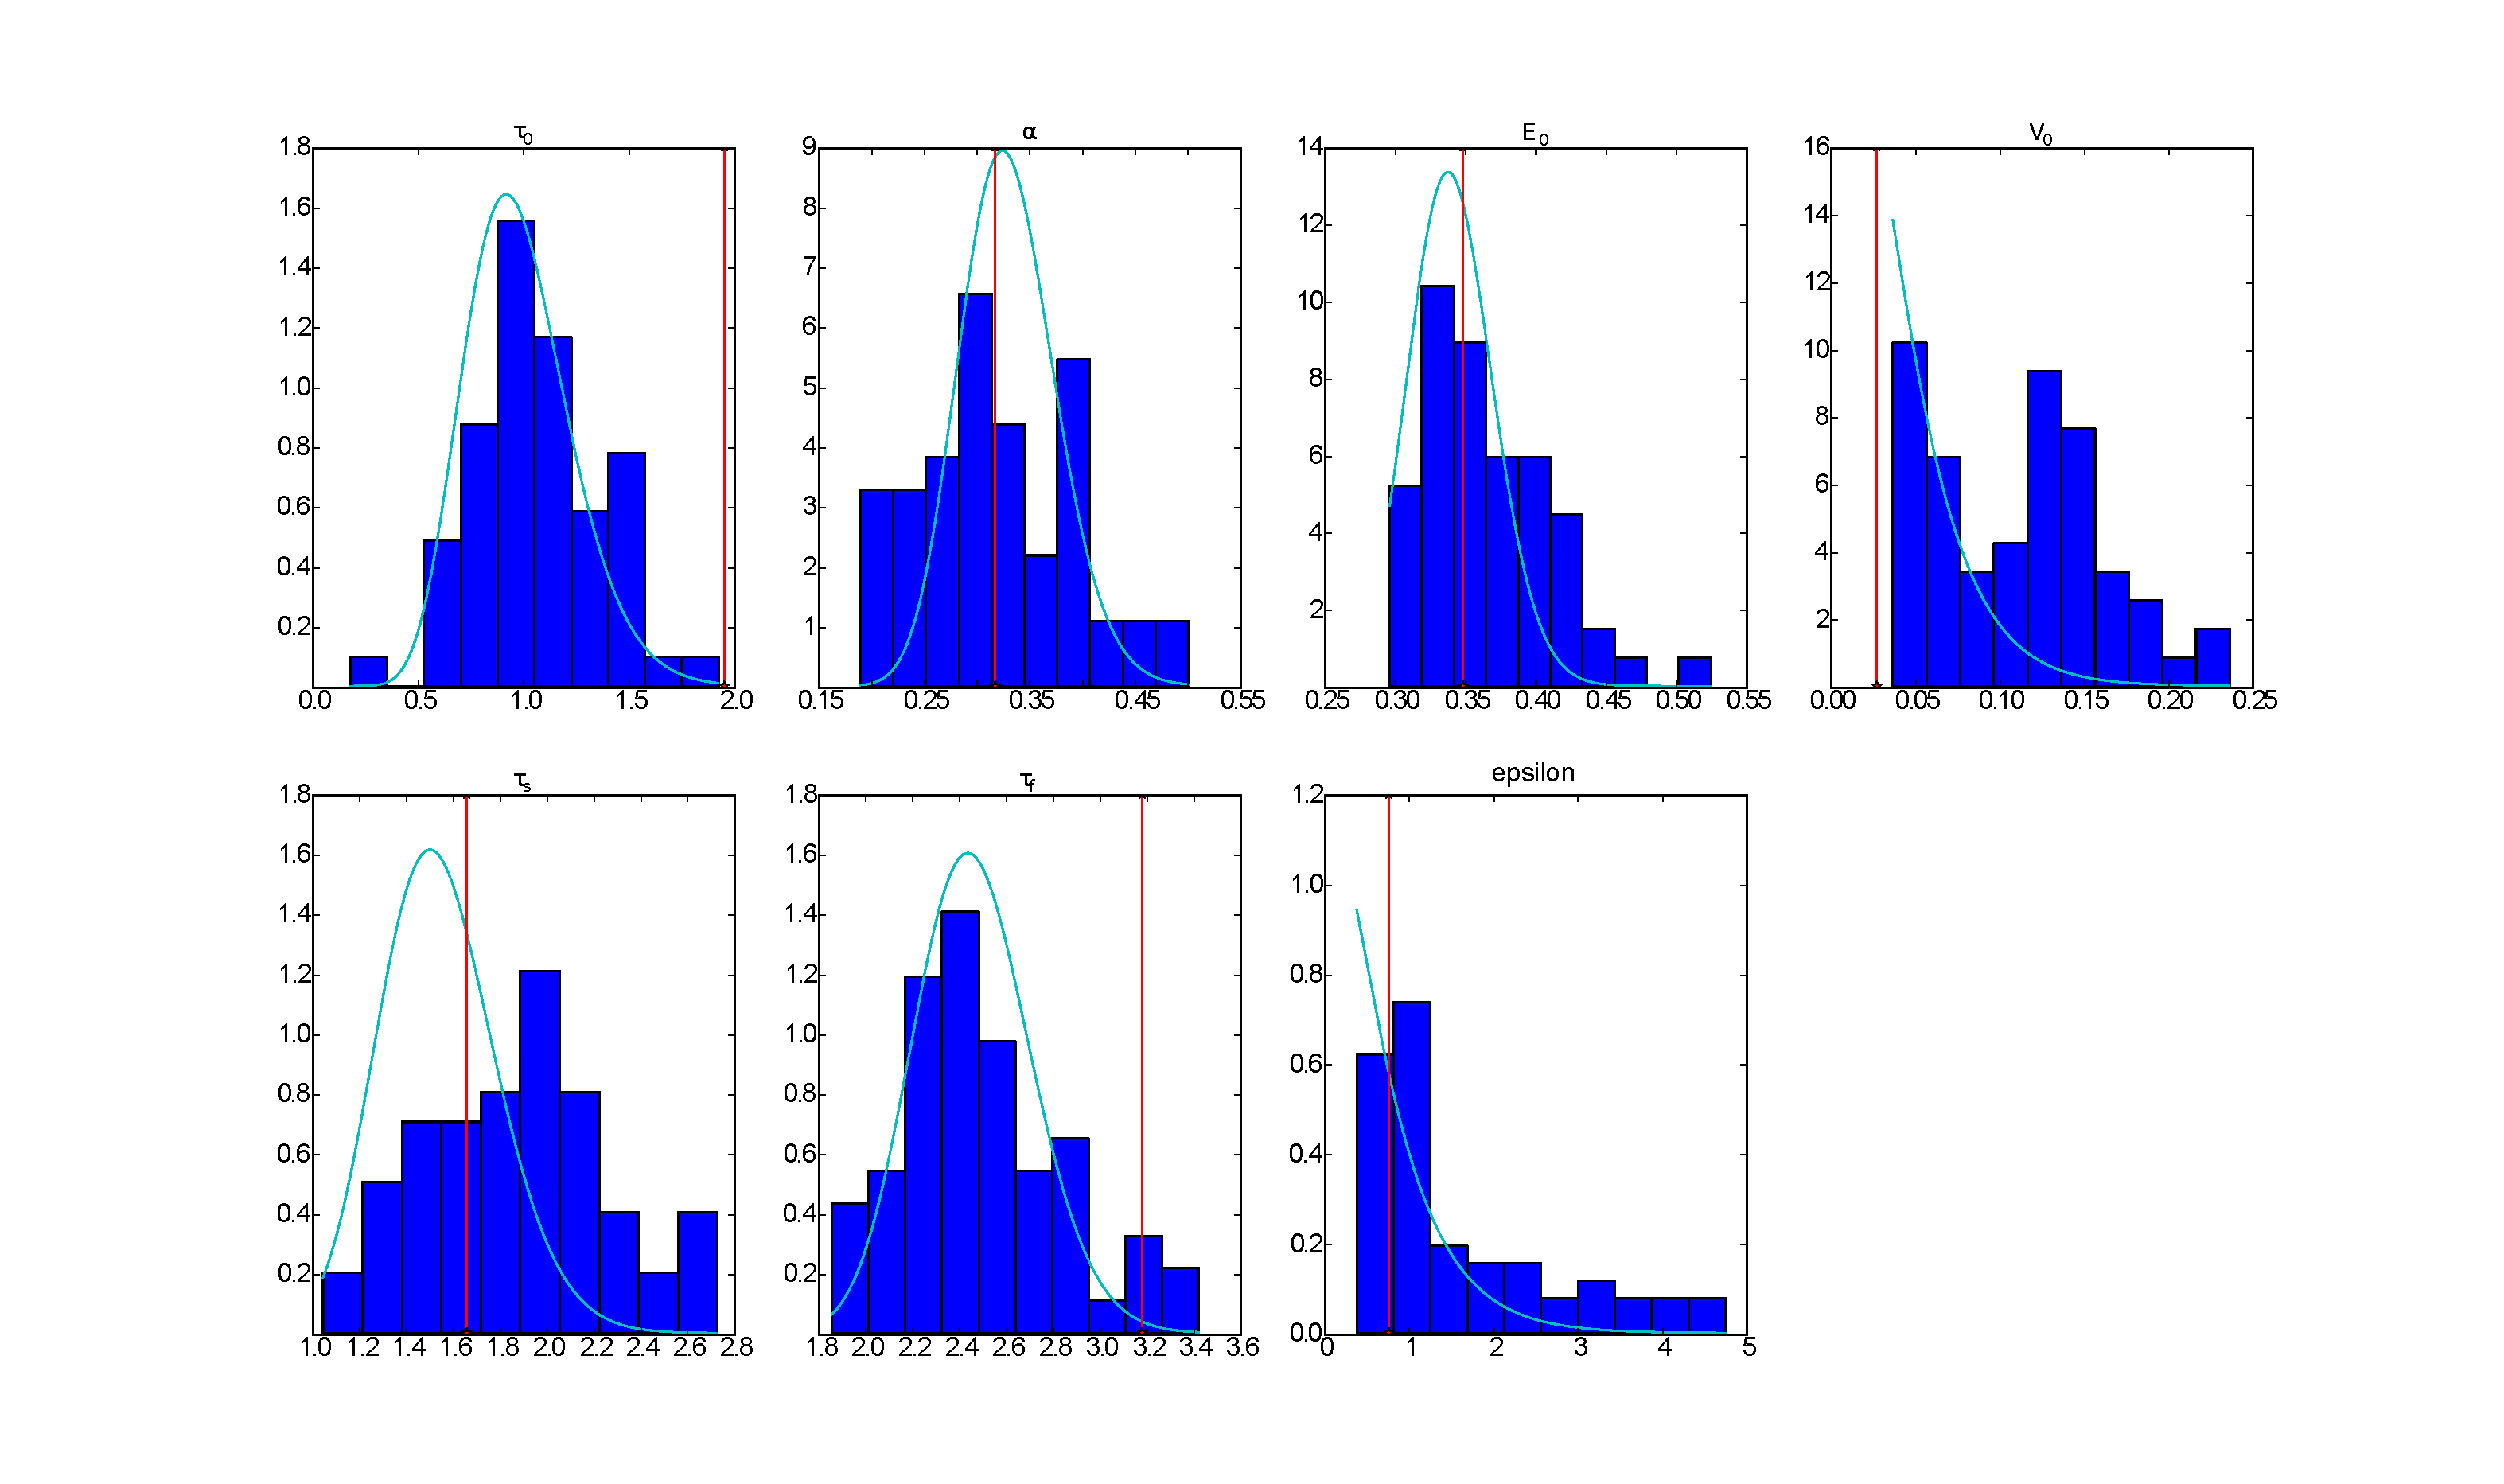
\includegraphics[clip=true,trim=5cm 2cm 5cm 2cm, width=.9\textwidth]{sec2hist}
\note{Histogram of estimated parameters.}
\note{Average SNR: $0.97$}
\note{Mutual Information greater than $0.15$.}
\end{figure}
\end{frame}

\subsection{Real FMRI Data}
\begin{frame}{SPM vs. Mutual Information Map}
\begin{columns}
\begin{column}{.5\textwidth}
\begin{figure}
\setcounter{subfigure}{0}

\subfigure[SPM Results]{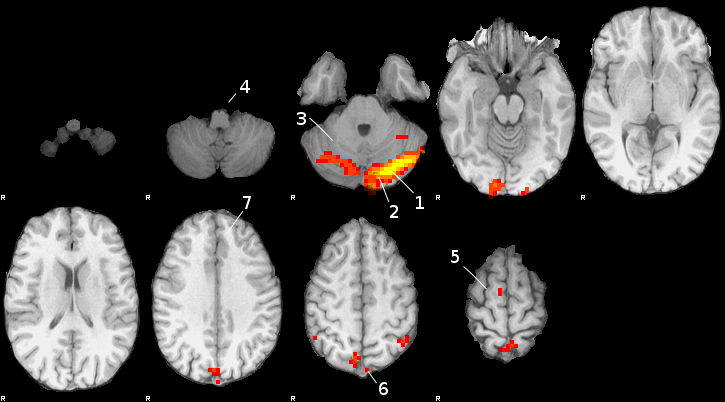
\includegraphics[width=.9\textwidth]{spm_hm}}
\subfigure{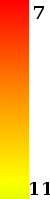
\includegraphics[width=.07\textwidth]{scale1}}
\note{SPM results. Units of activation are in Student's $t$-scores; higher 
        indicates higher assurance that the signal cannot have occurred 
        through noise alone.}
\label{fig:hm_canon_spm}
\end{figure}
\end{column}

\begin{column}{.5\textwidth}
\begin{figure}
\setcounter{subfigure}{1}
\subfigure[Particle Filter Results]{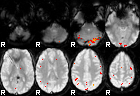
\includegraphics[width=.9\textwidth]{hm_mi_strict}}
\subfigure{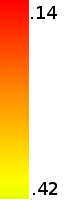
\includegraphics[height=1.5cm,width=.07\textwidth]{scale4}}
\note{Particle filter results. Units of activation are in mutual information;
    higher indicates more assured activation.}
\end{figure}
\end{column}
\end{columns}
\end{frame}

\begin{frame}{Particle Filter Results: Histogram}
\begin{figure}
\centering
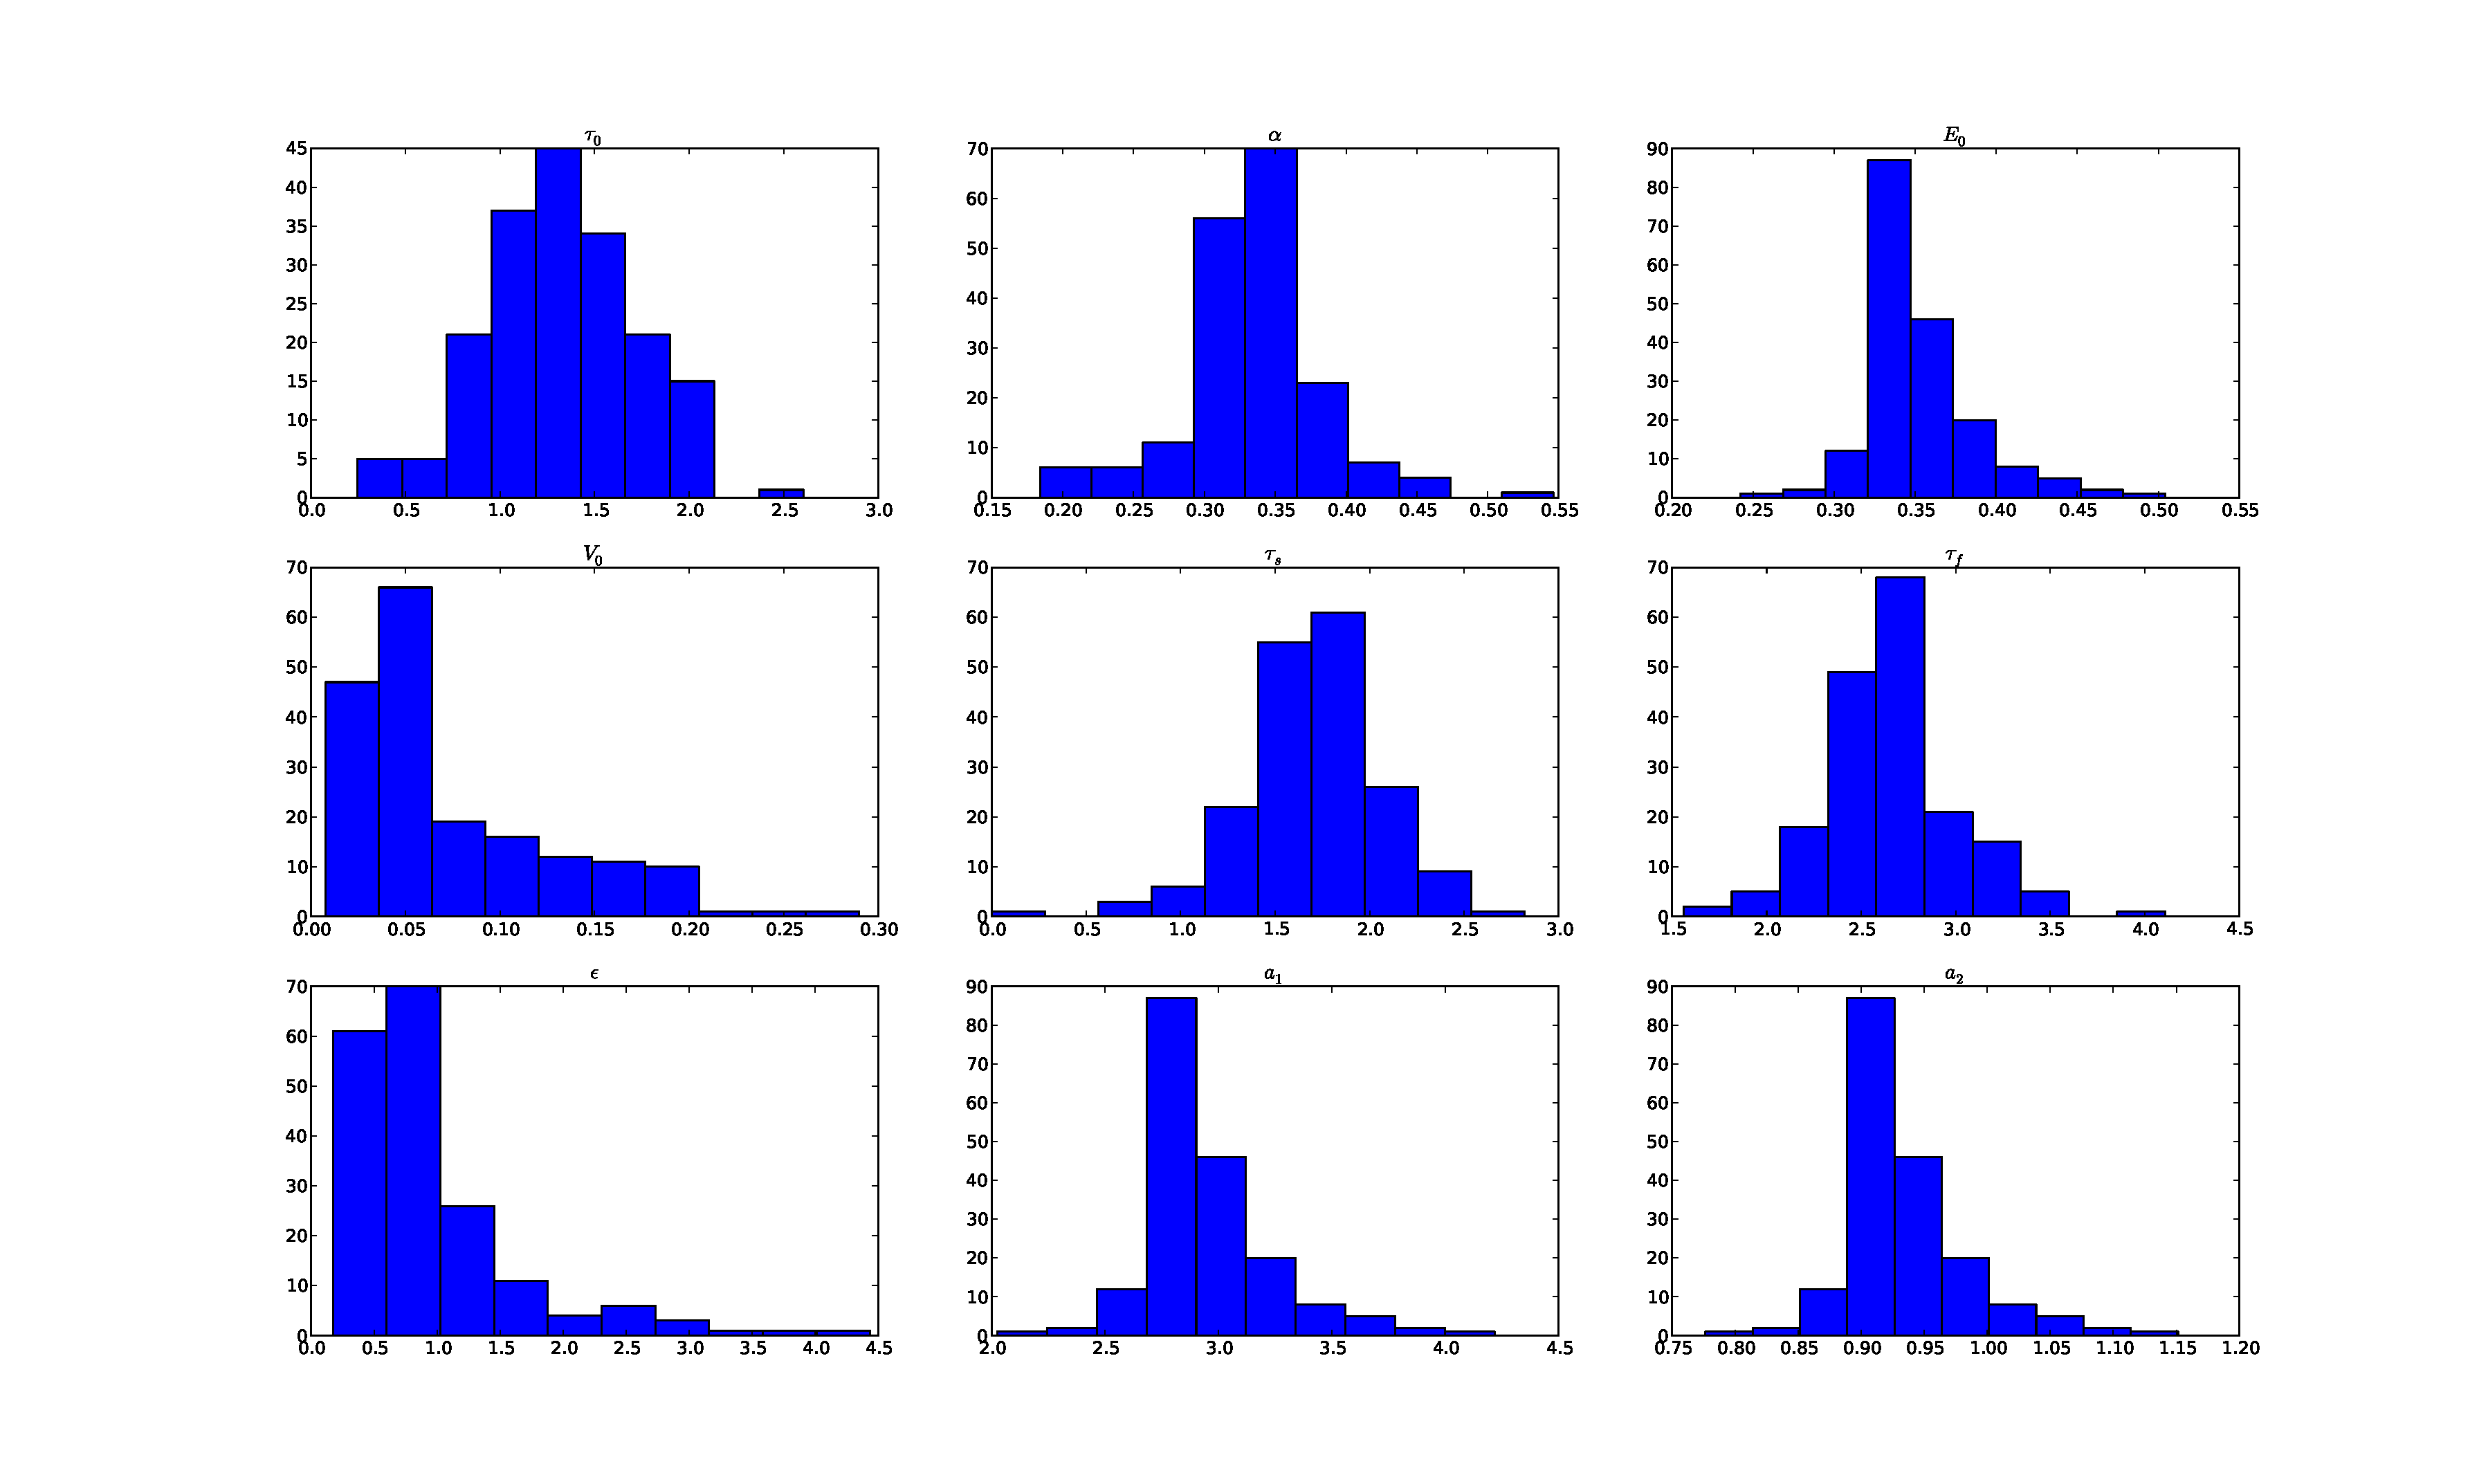
\includegraphics[clip=truew,trim=8cm 4cm 8cm 4cm,width=.8\textwidth]{realhist}
\note{Histogram of parameters in active regions ($M.I. > .15$).}
\end{figure}
\end{frame}

